
\documentclass[12pt,letterpaper]{article}

% Packages
\usepackage[utf8]{inputenc}
\usepackage{amsmath}
\usepackage{amssymb}
\usepackage{graphicx}
\usepackage{float}
\usepackage{geometry}
\usepackage{hyperref}

\usepackage{booktabs}
\usepackage{longtable}

\usepackage{pdfpages}

% Page margins
\geometry{margin=1in}

\begin{document}
% Document information
\begin{titlepage}
    \centering
    \vspace*{3cm}

    {\Huge\bfseries Refractive Index of a Prism\par}

    \vspace{2cm}

    {\Large Son Thanh Truong\par}
    {\Large Student ID: 100972716\par}
    \vspace{0.5cm}
    {\large Carleton University\par}
    {\large PHYS 2007\par}
    {\large Lab Section: C\par}
    {\large Lab Partner: Lauren Gilchrist\par}
    {\large Date of Report Submission: \today\par}
    
    
    \vfill

    {\large \today\par}
\end{titlepage}



%\maketitle

%\section{Introduction}

%Write your introduction here.

\section{Question 1}

The difference between Fresnel and Fraunhofer diffraction is that
the first one deals with when the observation plane is very close 
to the aperture, and deals with spherical wave fronts. The second
kind deals with "far field" approximation. That is when the aperture
to the plane distance is large. The far field approximation is
satisfied because the collimator was providing parallel incident light.
And also the telescope was focused at a far away object.
% Example equation
% \begin{equation}
%     F = ma
%     \label{eq:newton}
% \end{equation}

\section{Question 2}

Based on my observation, the pattern of the single slit was much
more simple. It was one thicker line, a bit thicker, in the middle.
Then the line's thickness and spacing were all even throughout.
For the double slit it was quite weird, it was almost exactly like
single slit except that there was a pattern of dimming in and out
that had a horizontal frequency about 10 times lower than the frequency
of the lines horizontally.

\section{Question 3}

When one is measuring many things are happening in this experiment that's
not just the reading error. The scale reading is +/-0.5' but other things
could introduce uncertainty for example how wide the opening slit is or what
technique was used to measure the data. Crosshair positioned in bright
or dark background could also affect the reading. Also if lab partners
had different glasses prescription, one sharp image for one could be blurry
for the other person.


\begingroup
\small
\setlength{\tabcolsep}{5pt}
\renewcommand{\arraystretch}{1.15}
\begin{longtable}{ccrrrrr}
\caption{Single-slit diffraction minima. All angles are in degrees. $\theta_{L,R}=\phi_{L,R}-\phi_0$.}\label{tab:diffraction-1}\\
\toprule
Trial & Order & Centre $\phi_0$ & Left $\phi_L$ & Right $\phi_R$ & $\theta_L$ & $\theta_R$ \\
\midrule
\endfirsthead
\toprule
Trial & Order & Centre $\phi_0$ & Left $\phi_L$ & Right $\phi_R$ & $\theta_L$ & $\theta_R$ \\
\midrule
\endhead
\midrule
\multicolumn{7}{r}{Continued on next page} \\
\endfoot
\bottomrule
\endlastfoot
1 & 1 & 84.867 & 85.000 & 84.750 & 0.133 & -0.117 \\
1 & 2 & 84.867 & 85.117 & 84.617 & 0.250 & -0.250 \\
1 & 3 & 84.867 & 85.317 & 84.500 & 0.450 & -0.367 \\
1 & 4 & 84.867 & 85.400 & 84.367 & 0.533 & -0.500 \\
1 & 5 & 84.867 & 85.550 & 84.217 & 0.683 & -0.650 \\
1 & 6 & 84.867 & 85.633 & 84.083 & 0.767 & -0.783 \\
\midrule
2 & 1 & 84.867 & 85.000 & 84.683 & 0.133 & -0.183 \\
2 & 2 & 84.867 & 85.067 & 84.517 & 0.200 & -0.350 \\
2 & 3 & 84.867 & 85.200 & 84.433 & 0.333 & -0.433 \\
2 & 4 & 84.867 & 85.350 & 84.283 & 0.483 & -0.583 \\
2 & 5 & 84.867 & 85.500 & 84.167 & 0.633 & -0.700 \\
2 & 6 & 84.867 & 85.583 & 84.083 & 0.717 & -0.783 \\
\midrule
3 & 1 & 84.850 & 85.000 & 84.700 & 0.150 & -0.150 \\
3 & 2 & 84.850 & 85.100 & 84.600 & 0.250 & -0.250 \\
3 & 3 & 84.850 & 85.250 & 84.500 & 0.400 & -0.350 \\
3 & 4 & 84.850 & 85.350 & 84.350 & 0.500 & -0.500 \\
3 & 5 & 84.850 & 85.500 & 84.200 & 0.650 & -0.650 \\
3 & 6 & 84.850 & 85.667 & 84.150 & 0.817 & -0.700 \\
\end{longtable}

\begin{longtable}{ccrrrrr}
\caption{Double-slit diffraction minima. All angles are in degrees. $\theta_{L,R}=\phi_{L,R}-\phi_0$.}\label{tab:diffraction-2}\\
\toprule
Trial & Order & Centre $\phi_0$ & Left $\phi_L$ & Right $\phi_R$ & $\theta_L$ & $\theta_R$ \\
\midrule
\endfirsthead
\toprule
Trial & Order & Centre $\phi_0$ & Left $\phi_L$ & Right $\phi_R$ & $\theta_L$ & $\theta_R$ \\
\midrule
\endhead
\midrule
\multicolumn{7}{r}{Continued on next page} \\
\endfoot
\bottomrule
\endlastfoot
1 & 1 & 84.900 & 85.250 & 84.433 & 0.350 & -0.467 \\
1 & 2 & 84.900 & 85.500 & 84.150 & 0.600 & -0.750 \\
1 & 3 & 84.900 & 85.933 & 83.733 & 1.033 & -1.167 \\
\midrule
2 & 1 & 85.750 & 86.017 & 85.450 & 0.267 & -0.300 \\
2 & 2 & 85.750 & 86.500 & 85.000 & 0.750 & -0.750 \\
2 & 3 & 85.750 & 86.917 & 84.767 & 1.167 & -0.983 \\
\end{longtable}

\begin{longtable}{ccrrrrr}
\caption{Double-slit interference maxima. All angles are in degrees. $\theta_{L,R}=\phi_{L,R}-\phi_0$.}\label{tab:diffraction-3}\\
\toprule
Trial & Order & Centre $\phi_0$ & Left $\phi_L$ & Right $\phi_R$ & $\theta_L$ & $\theta_R$ \\
\midrule
\endfirsthead
\toprule
Trial & Order & Centre $\phi_0$ & Left $\phi_L$ & Right $\phi_R$ & $\theta_L$ & $\theta_R$ \\
\midrule
\endhead
\midrule
\multicolumn{7}{r}{Continued on next page} \\
\endfoot
\bottomrule
\endlastfoot
1 & 1 & 84.850 & 84.983 & 84.717 & 0.133 & -0.133 \\
1 & 2 & 84.850 & 85.017 & 84.583 & 0.167 & -0.267 \\
1 & 3 & 84.850 & 85.250 & 84.933$^{\dagger}$ & 0.400 & 0.083$^{\dagger}$ \\
1 & 4 & 84.850 & 85.367 & 84.783$^{\dagger}$ & 0.517 & -0.067$^{\dagger}$ \\
1 & 5 & 84.850 & 85.517 & 84.150 & 0.667 & -0.700 \\
1 & 6 & 84.850 & 85.667 & 84.117 & 0.817 & -0.733 \\
\midrule
2$^{*}$ & 1 & 84.850 & 84.983 & \textemdash & 0.133 & \textemdash \\
2$^{*}$ & 2 & 84.850 & 85.017 & \textemdash & 0.167 & \textemdash \\
2$^{*}$ & 3 & 84.850 & 85.250 & \textemdash & 0.400 & \textemdash \\
2$^{*}$ & 4 & 84.850 & 85.367 & \textemdash & 0.517 & \textemdash \\
2$^{*}$ & 5 & 84.850 & 85.517 & \textemdash & 0.667 & \textemdash \\
2$^{*}$ & 6 & 84.850 & 85.667 & \textemdash & 0.817 & \textemdash \\
\midrule
3 & 1 & 85.467 & 85.550 & 85.283 & 0.083 & -0.183 \\
3 & 2 & 85.467 & 85.733 & 85.167 & 0.267 & -0.300 \\
3 & 3 & 85.467 & 85.850 & 85.000 & 0.383 & -0.467 \\
3 & 4 & 85.467 & 85.983 & 84.900 & 0.517 & -0.567 \\
3 & 5 & 85.467 & 86.150 & 84.767 & 0.683 & -0.700 \\
3 & 6 & 85.467 & 86.283 & 84.633 & 0.817 & -0.833 \\
\midrule
\multicolumn{7}{l}{$^{\dagger}$ Right reading questionable: transcription or fringe order unverified.} \\
\multicolumn{7}{l}{$^{*}$ Incomplete trial; not used for paired left/right analysis.} \\
\end{longtable}

\endgroup

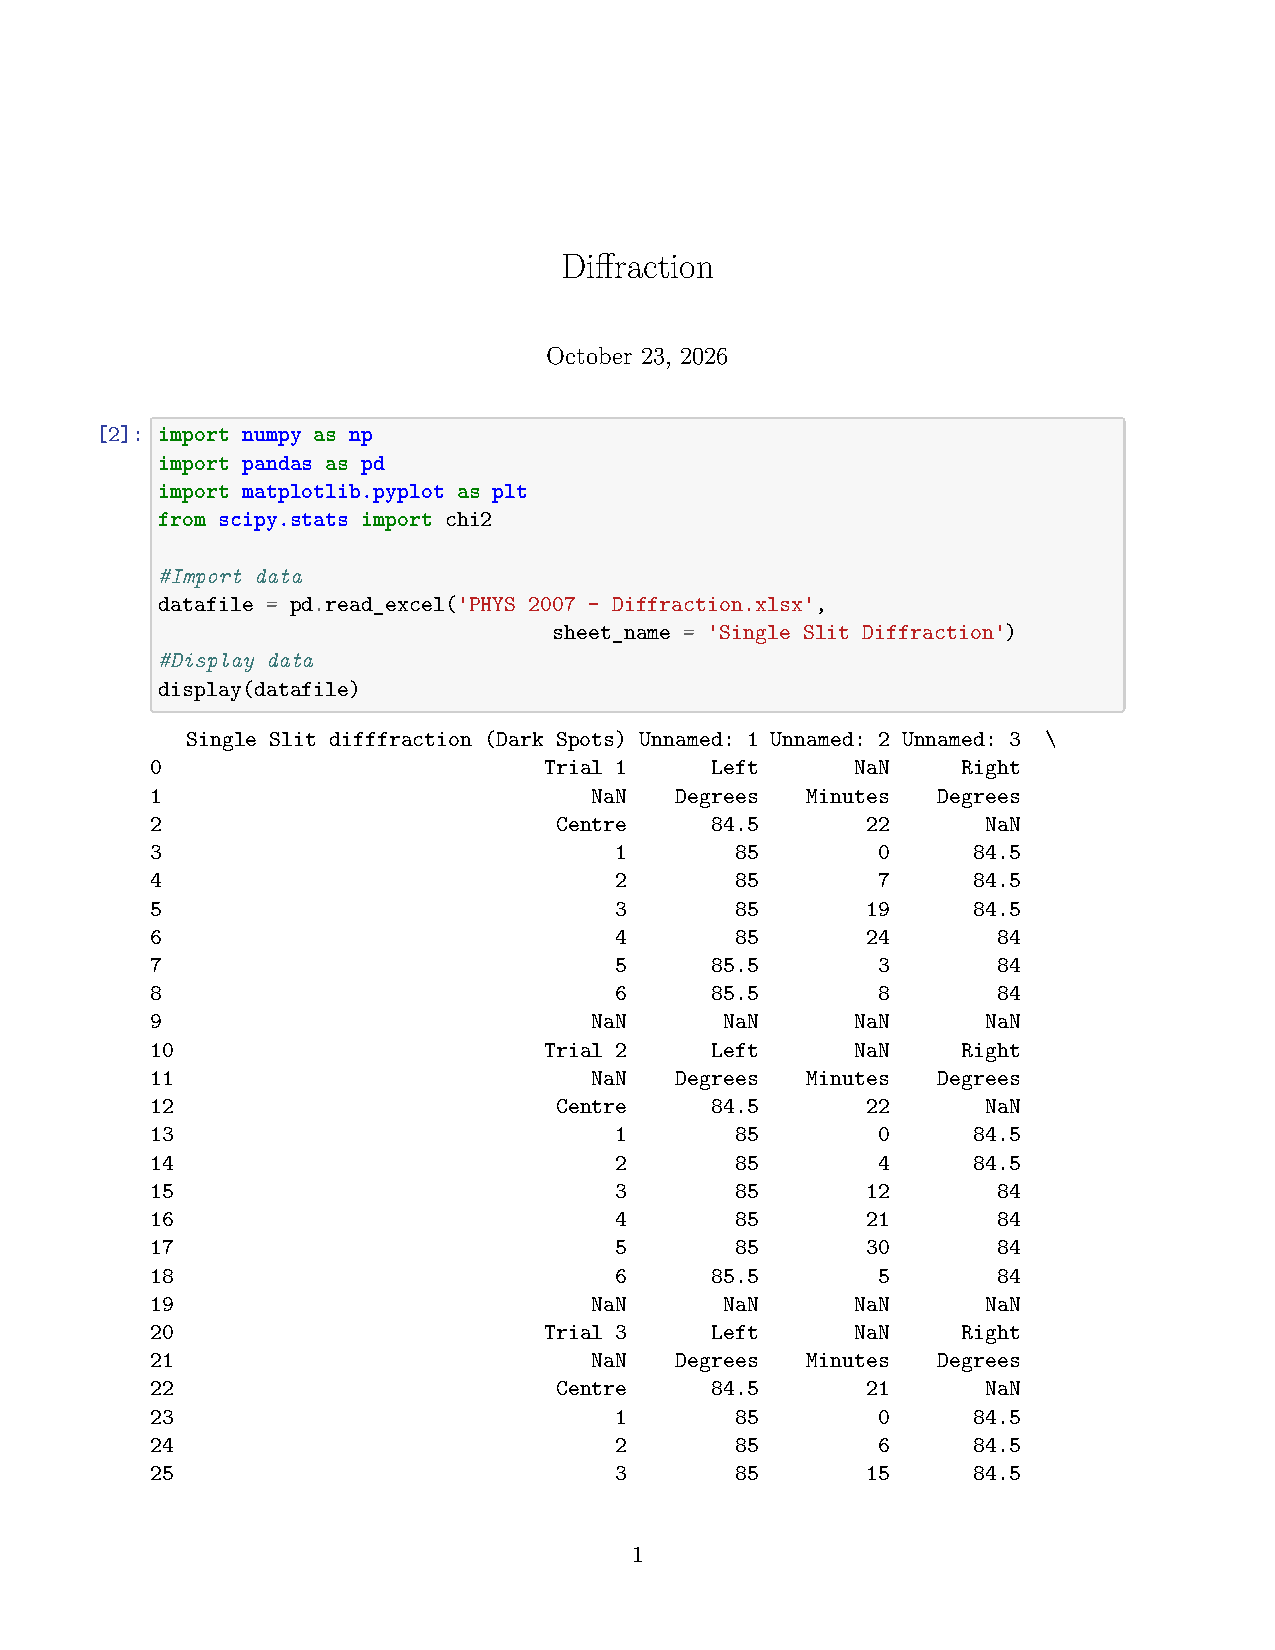
\includepdf[pages=-]{Diffraction.pdf}

\end{document}
